\documentclass{article}
\usepackage{tikz}
\usetikzlibrary{calc} % enables coordinate math

\begin{document}

% Basic coordinate calculation demo
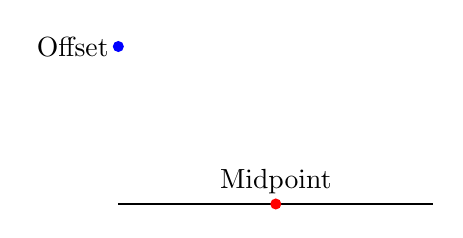
\begin{tikzpicture}[scale=1]

  % --- Define base points ---
  \coordinate (A) at (0,0);
  \coordinate (B) at (4,0);

  % --- Draw line AB ---
  \draw[thick] (A) -- (B);

  % --- Midpoint between A and B ---
  \coordinate (M) at ($(A)!0.5!(B)$);
  \fill[red] (M) circle (2pt);
  \node[above] at (M) {Midpoint};

  % --- Offset point from A ---
  \coordinate (O) at ($(A)+(0,2)$);
  \fill[blue] (O) circle (2pt);
  \node[left] at (O) {Offset};

\end{tikzpicture}

\end{document}
